\subsection{Freeciv}
\begin{frame}
	\frametitle{Freeciv}

	\begin{columns}
		\column{0.75\textwidth}
		
		\begin{itemize}
			\item<1-> Turn-based strategy videogame.
			\item<2-> Created by students of Aarhus University.
			\item<3-> Today developed by a open source community.
		\end{itemize}
		
		\column{0.25\textwidth}
		\centering
		
\includegraphics[width=0.8\textwidth]{images/freeciv.png}
	\end{columns}
\end{frame}

\subsection{Game design}
\begin{frame}
	\frametitle{Game design}
	\begin{itemize}
		\item<1-> Player controls a group of settlers in 4000 B.C.
		\item<2-> 5 game ends:
		\begin{itemize}
			\item<3-> Domination victory.
			\item<3-> Science victory.
			\item<3-> Religion victory.
			\item<3-> Culture victory.
			\item<3-> Score victory.
		\end{itemize}
	\end{itemize}
\end{frame}

\subsection{Types of terrains}
\begin{frame}
\frametitle{Freeciv terrains}
	\begin{columns}
		\column{0.20\textwidth}
		\centering 
\includegraphics[width=0.7\textwidth]{images/grassland.png}
		
		\column{0.80\textwidth}
		\begin{itemize}
			\item Grassland: Common. Units can move easy.
		\end{itemize}
	\end{columns}

	\vspace{1em}
	
	\begin{columns}
		\column{0.20\textwidth}
		\centering 
\includegraphics[width=0.7\textwidth]{images/plains.png}
		
		\column{0.80\textwidth}
		\begin{itemize}
			\item Plains: You can create roads on this cells.
		\end{itemize}
	\end{columns}

	\vspace{1em}
	
	\begin{columns}
		\column{0.20\textwidth}
		\centering 
\includegraphics[width=0.7\textwidth]{images/hills.png}
		
		\column{0.80\textwidth}
		\begin{itemize}
			\item Hills: Units move slowly. +200\% defense bonus.
		\end{itemize}
	\end{columns}

	\vspace{1em}
	
	\begin{columns}
		\column{0.20\textwidth}
		\centering 
\includegraphics[width=0.7\textwidth]{images/forest.png}
		
		\column{0.80\textwidth}
		\begin{itemize}
			\item Forest: +1 production unit. +150\% defense bonus.
		\end{itemize}
	\end{columns}
\end{frame}

\begin{frame}
\frametitle{Freeciv terrains}
	\begin{columns}
		\column{0.20\textwidth}
		\centering 
\includegraphics[width=0.7\textwidth]{images/jungle.png}
		
		\column{0.80\textwidth}
		\begin{itemize}
			\item Jungle: +4 production units with gems/fruit bonus.
		\end{itemize}
	\end{columns}
	
	\vspace{1em}
	
	\begin{columns}
		\column{0.20\textwidth}
		\centering 
\includegraphics[width=0.7\textwidth]{images/mountains.png}
		
		\column{0.80\textwidth}
		\begin{itemize}
			\item Mountains: +300\% defense bonus.
		\end{itemize}
	\end{columns}
	
	\vspace{1em}
	
	\begin{columns}
		\column{0.20\textwidth}
		\centering 
\includegraphics[width=0.7\textwidth]{images/desert.png}
		
		\column{0.80\textwidth}
		\begin{itemize}
			\item Desert: +3 production units with oasis bonus.
		\end{itemize}
	\end{columns}
	
	\vspace{1em}
	
	\begin{columns}
		\column{0.20\textwidth}
		\centering 
\includegraphics[width=0.7\textwidth]{images/swamp.png}
		
		\column{0.80\textwidth}
		\begin{itemize}
			\item Swamp: Fast irrigating. +5/9 production units with peat and spice bonus.
		\end{itemize}
	\end{columns}
\end{frame}

\begin{frame}
\frametitle{Freeciv terrains}
	\begin{columns}
		\column{0.20\textwidth}
		\centering 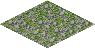
\includegraphics[width=0.7\textwidth]{images/tundra.png}
		
		\column{0.80\textwidth}
		\begin{itemize}
			\item Tundra: Only create roads.
		\end{itemize}
	\end{columns}
	
	\vspace{1em}
	
	\begin{columns}
		\column{0.20\textwidth}
		\centering 
\includegraphics[width=0.7\textwidth]{images/glacier.png}
		
		\column{0.80\textwidth}
		\begin{itemize}
			\item Glacier: All the units cannot pass through.
		\end{itemize}
	\end{columns}
	
	\vspace{1em}
	
	\begin{columns}
		\column{0.20\textwidth}
		\centering 
\includegraphics[width=0.7\textwidth]{images/sea.png}
		
		\column{0.80\textwidth}
		\begin{itemize}
			\item Sea: All type of boats can pass through.
		\end{itemize}
	\end{columns}
	
	\vspace{1em}
	
	\begin{columns}
		\column{0.20\textwidth}
		\centering 
\includegraphics[width=0.7\textwidth]{images/ocean.png}
		
		\column{0.80\textwidth}
		\begin{itemize}
			\item Ocean: Only big ships can pass through.
		\end{itemize}
	\end{columns}
\end{frame}